\documentclass{article}

\usepackage{graphicx}
\usepackage{tikz}
\usepackage{tikzsymbols}
\usetikzlibrary{calc,patterns,shapes.geometric}
\pagestyle{empty}
\usepackage[margin=0pt]{geometry}
\geometry{papersize={14in,12in}}

\def\centerarc[#1](#2)(#3:#4:#5){\draw[#1] ($(#2)+({#5*cos(#3)},{#5*sin(#3)})$) arc (#3:#4:#5);}

\begin{document}
	\begin{figure}
		\centering
		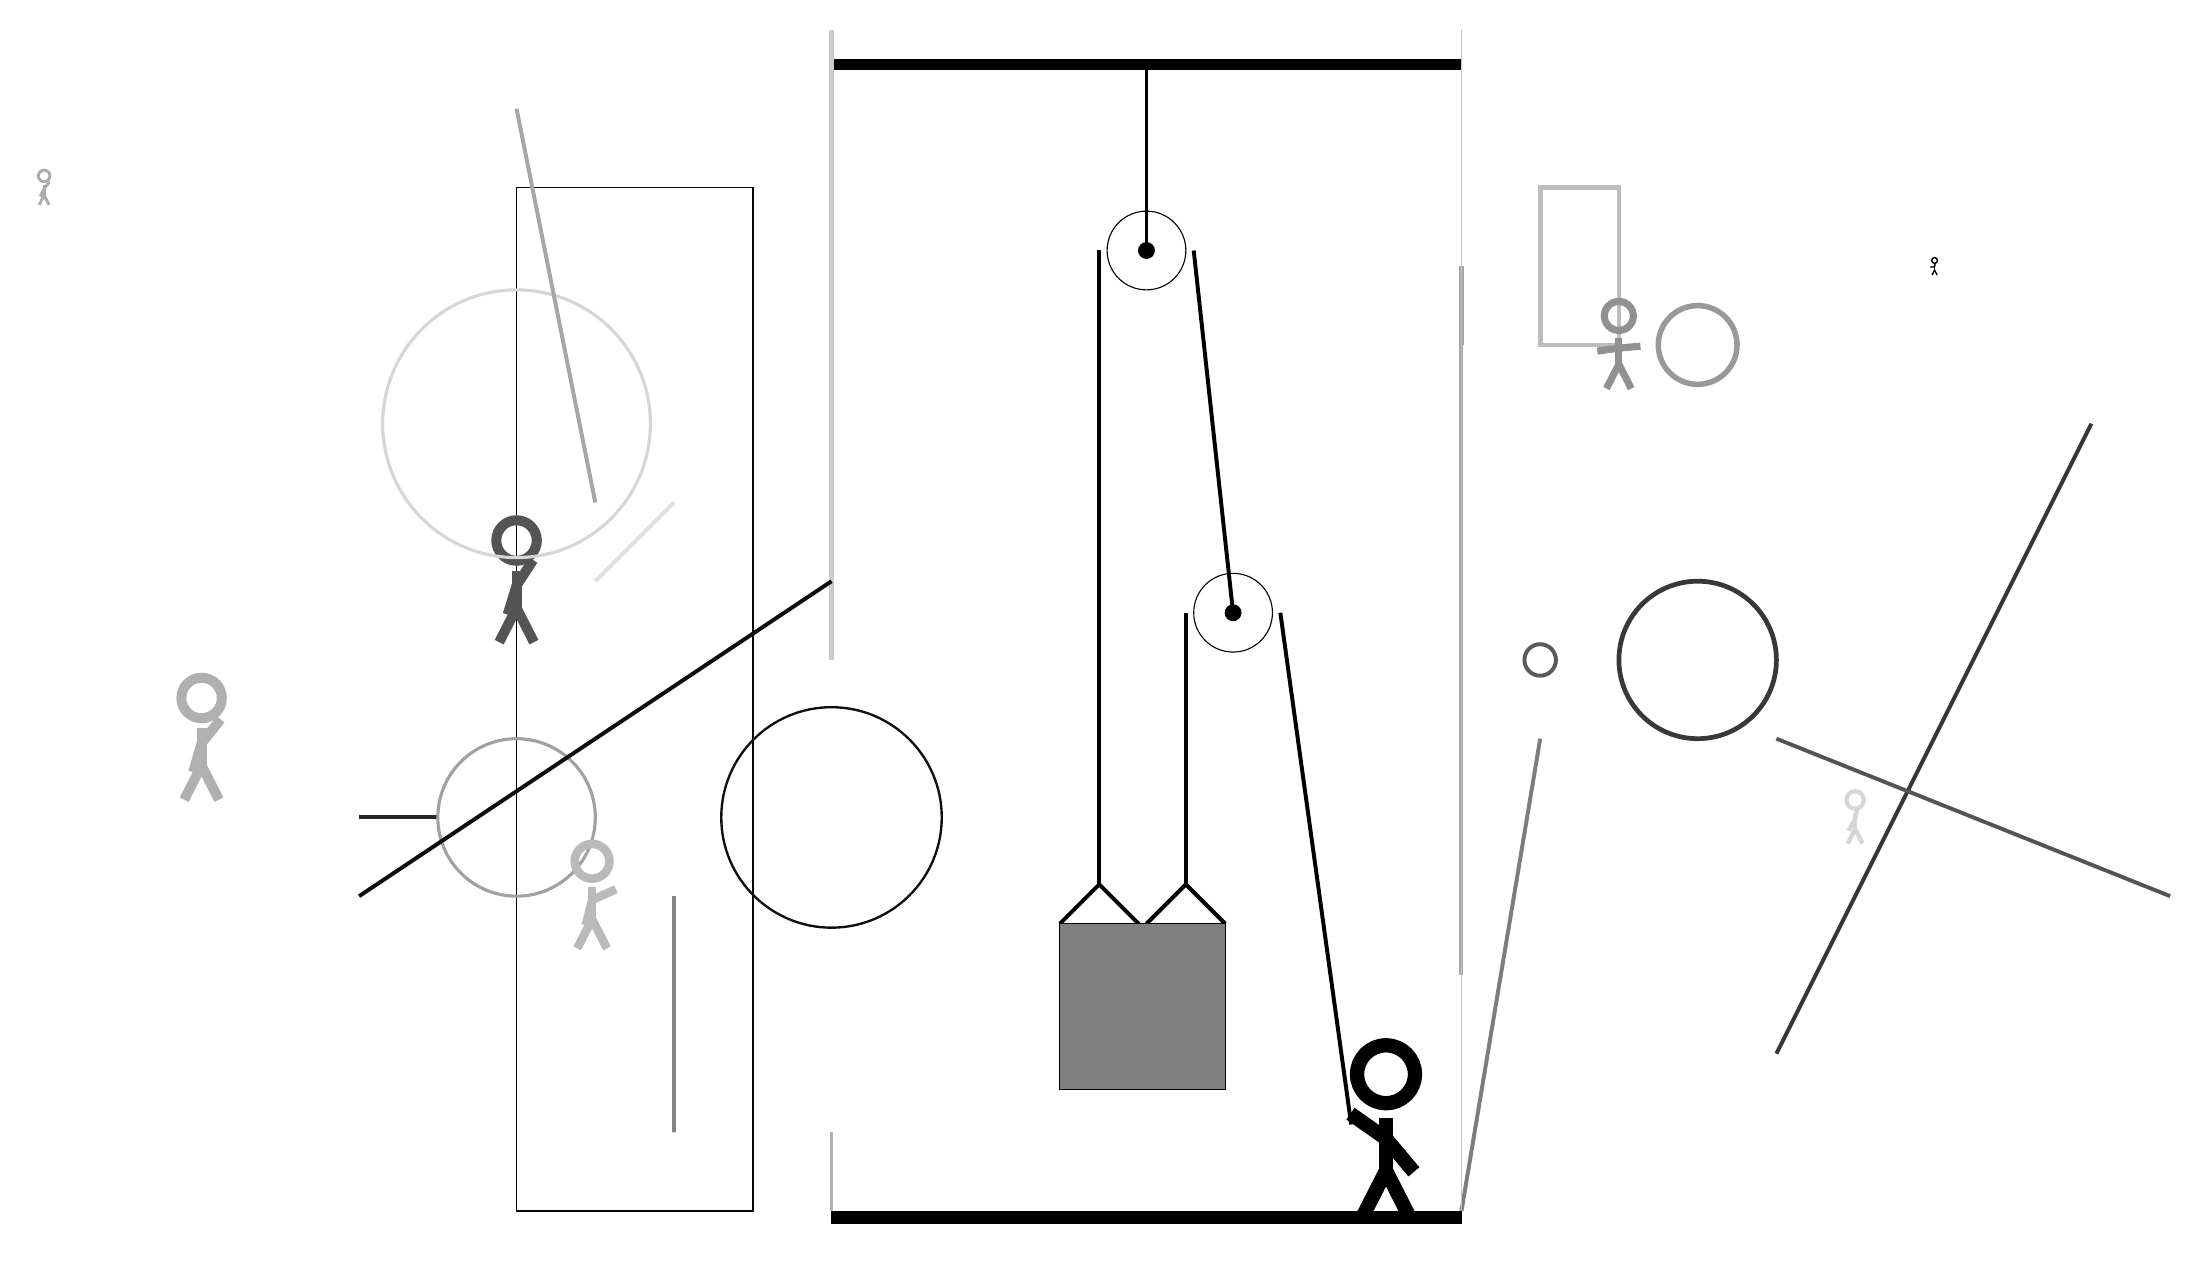
\begin{tikzpicture}
			%%%%% START %%%%%
			
			\draw[fill=black] (-2, 11.5) rectangle (6, 11.625);
			
			\draw (2, 9.2) circle (0.5);
			\draw[fill=black] (2, 9.2) circle (0.1);
			\draw[thick] (2, 9.2) -- (2, 11.5);
			
			\draw (3.1, 4.6) circle (0.5);
			\draw[fill=black] (3.1, 4.6) circle (0.1);
			
			\draw[line width = 0.5mm]  (0.9, 0.65) -- (1.4, 1.15) -- (1.9, 0.65);
			\draw[line width = 0.5mm]  (2.0, 0.65) -- (2.5, 1.15) -- (3.0, 0.65);
			\draw[fill=black!50] (0.9, 0.65) rectangle (3.0, -1.45);
			
			\draw[line width=0.5mm, color=black!79](10, -1) -- (14, 7);
			
			\draw[line width=0.6mm, color=black!20] (-2, 4) rectangle (-2, 12);
			\draw[line width=0.2mm, color=black!98] (-3, -3) rectangle (-6, 10);
			\draw [line width=0.6mm, color=black!78](9, 4) circle (1.0);
			
			\node[line width=0.3mm, color=black!67] at (-6, 5) {\Strichmaxerl[7][73][57]};
			
			\draw[line width=0.5mm, color=black!51](6, -3) -- (7, 3);
			\draw[line width=0.5mm, color=black!67](10, 3) -- (15, 1);
			
			\draw[line width=0.6mm, color=black!37] (6, 9) rectangle (6, 8);
			\draw[line width=0.5mm, color=black!12](-5, 5) -- (-4, 6);
			
			\draw[line width=0.5mm, color=black!85](-7, 2) -- (-8, 2);
			\draw [line width=0.4mm, color=black!16](-6, 7) circle (1.7);
			\node[line width=0.5mm, color=black!97] at (12, 9) {\Strichmaxerl[1][3][81]};
			\draw[line width=0.6mm, color=black!26] (8, 10) rectangle (7, 8);
			\draw [line width=0.4mm, color=black!37](-6, 2) circle (1.0);
			\draw[line width=0.5mm, color=black!30](-2, -2) -- (-2, -3);
			\node[line width=0.2mm, color=black!43] at (8, 8) {\Strichmaxerl[5][8][5]};
			
			\node[line width=0.7mm, color=black!33] at (-12, 10) {\Strichmaxerl[2][63][52]};
			
			\draw [line width=0.5mm, color=black!65](7, 4) circle (0.2);
			\draw[line width=0.5mm, color=black!36](-7, 6) -- (-7, 6);
			\node[line width=0.7mm, color=black!16] at (11, 2) {\Strichmaxerl[3][60][79]};
			\node[line width=0.6mm, color=black!27] at (-5, 1) {\Strichmaxerl[6][76][24]};
			
			\node[line width=0.3mm, color=black!31] at (-10, 3) {\Strichmaxerl[7][74][51]};
			
			\draw [line width=0.7mm, color=black!40](9, 8) circle (0.5);
			\draw[line width=0.5mm, color=black!48] (-4, 1) rectangle (-4, -2);
			\draw [line width=0.3mm, color=black!94](-2, 2) circle (1.4);
			\draw[line width=0.5mm, color=black!34](6, 0) -- (6, 9);
			\draw[line width=0.5mm, color=black!35](-6, 11) -- (-5, 6);
			\draw[line width=0.5mm, color=black!94](-2, 5) -- (-8, 1);
			\draw[line width=0.2mm, color=black!24] (6, 12) rectangle (6, -3);
			
			
			\draw[line width = 0.5mm] (1.4, 9.2) -- (1.4, 1.15);
			\centerarc[line width = 0.5mm](2, 9.2)(0:180:0.6);
			\draw[line width = 0.5mm] (2.6, 9.2) -- (3.1, 4.6);
			\draw[line width = 0.5mm] (2.5, 4.6) -- (2.5, 1.15);
			\centerarc[line width = 0.5mm](3.1, 4.6)(0:180:0.6);
			\draw[line width = 0.5mm] (3.7, 4.6) -- (4.6, -1.9);
			
			\node at (5, -2) {\Strichmaxerl[10][-35][-50]};
			
			\draw[fill=black] (-2, -3) rectangle (6, -3.15);
			
			%%%%% END %%%%%
		\end{tikzpicture}
	\end{figure}	
\end{document}